\section{Data Requirements Analysis}

\subsection{Choice of Topic and Research of Related Systems}
For this assignment, we choose to design an \textbf{Electronic Medical Record and Appointment system}. To establish a baseline for our proposed system, we have analyzed a relevant systems in the Vietnamese healthcare market: YouMed.

\textbf{Link:} \url{https://youmed.vn/} \par
\textbf{Business Process Analysis:} \par
YouMed operates on a dual-sided marketplace model, effectively bridging the patient's need for accessible care with the medical provider's need for operational efficiency. There are two platforms serving two user groups: \textbf{YouMed} for Patients and \textbf{Doctor Workspace} for Medical Providers.
\begin{enumerate}
    \item \textbf{Patient Workflow (YouMed App / Web)}
    \begin{itemize}
        \item \textbf{Phase 1: Account Registration and Profile Setup} \par
        \textbf{Primary Account Creation:} The user registers by providing all compulsory attributes: full name, phone number, date of birth, and a secure password. To complete their profile, the patient can optionally input their SSN, gender, email, ethnicity, health insurance number, detailed address (province/city, district/county, ward/commune, specific address), job, and a referrer code. \par
        \begin{figure}[H]
            \centering
            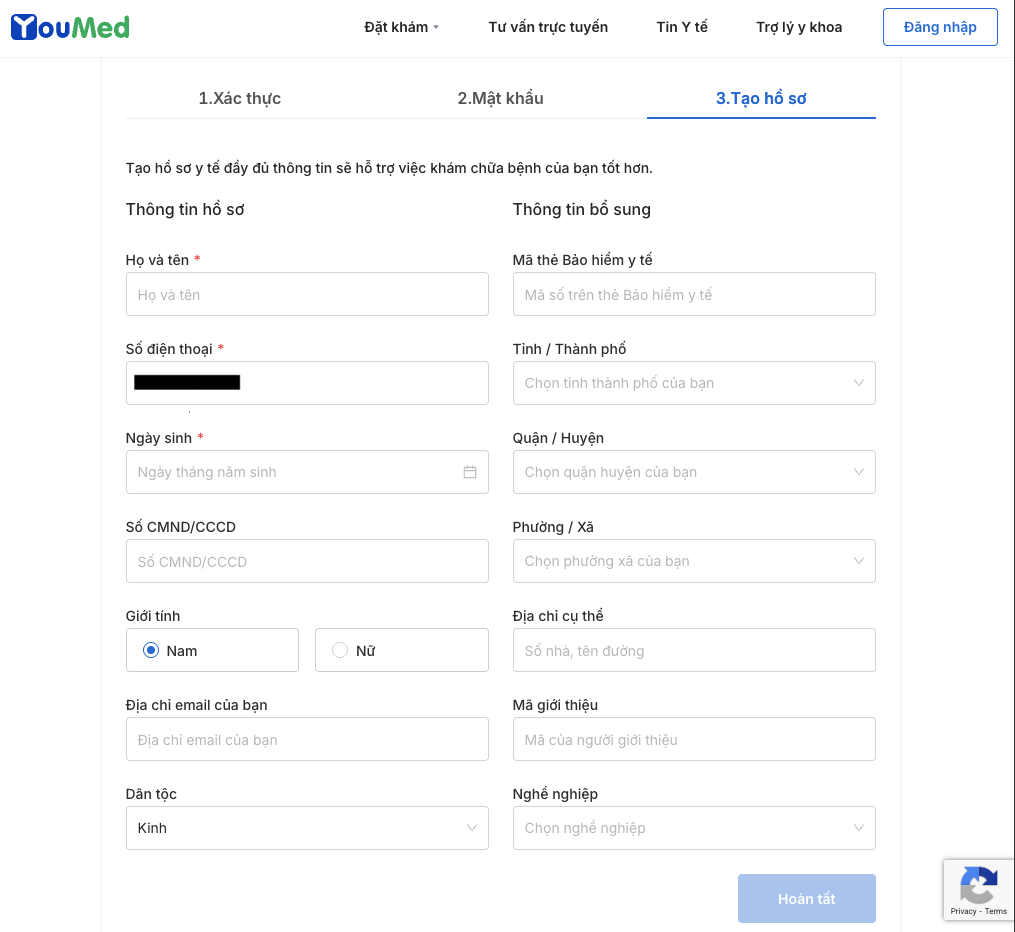
\includegraphics[width=0.8\linewidth]{images/youmed/youmed1.png}
            \caption{YouMed Account Registration}
            \label{fig:youmed_registration}
        \end{figure}
            
        \textbf{Creating Dependent Profiles (Optional):} If the user manages healthcare for family members, they can create dependent profiles. They input the standard patient details for the dependent and select a relationship attribute (e.g., father, mother, child) to link the dependent to the primary account.
        \begin{figure}[h]
            \centering
            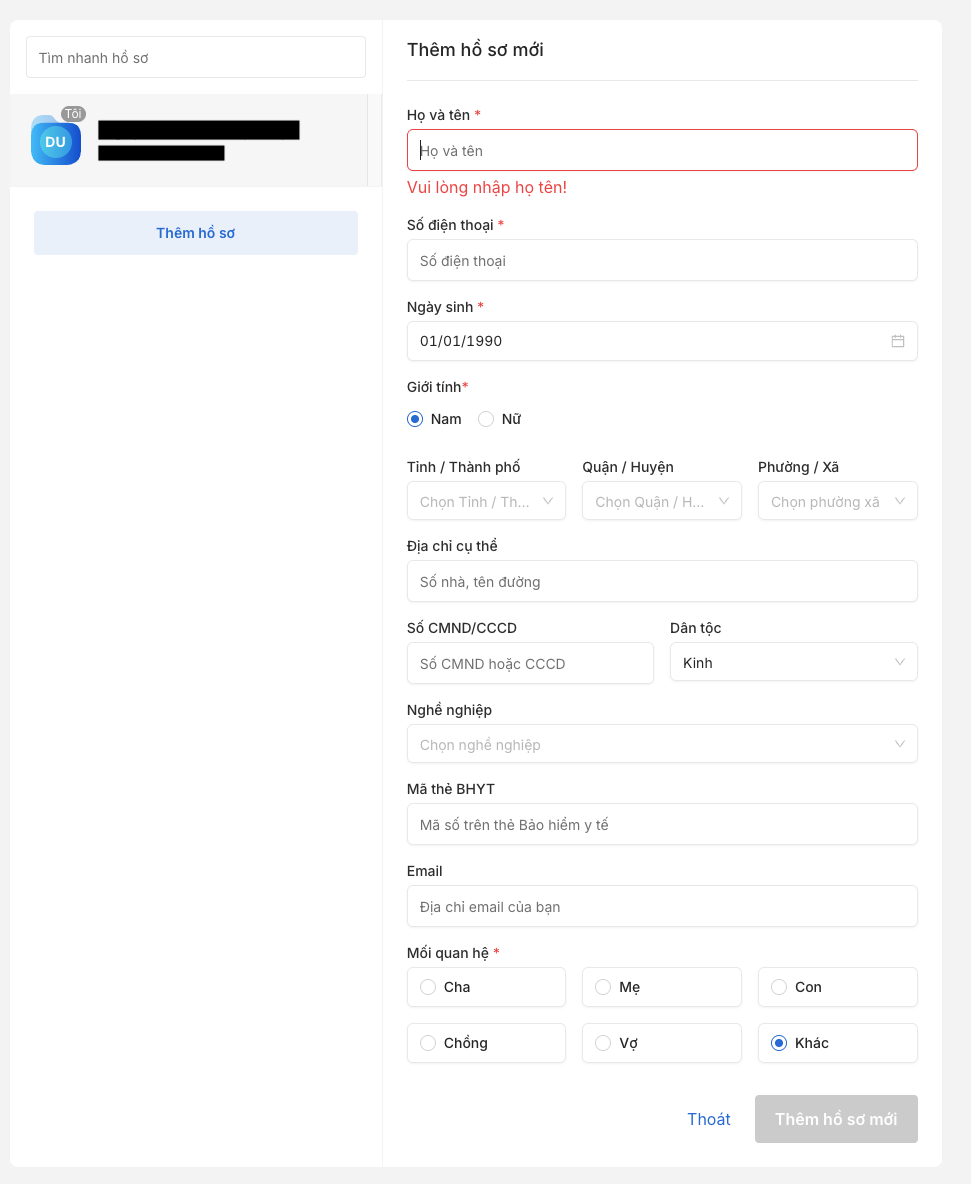
\includegraphics[width=0.7\linewidth]{images/youmed/youmed2.png}
            \caption{Creating Dependent Profiles}
            \label{fig:youmed_registration}
        \end{figure}

        \item \textbf{Phase 2: Routing and Scheduling} \par
        \textbf{Choosing the Booking Path:} The user selects one of four specific workflows based on their healthcare needs: booking a specific doctor, a hospital visit, a clinic appointment, or a vaccination schedule. \par
        \begin{figure}[H]
            \centering
            
\includegraphics[width=0.25\linewidth]{images/youmed/youmed3.png}
            \caption{Four Booking Paths}
            \label{fig:youmed_booking_path}
        \end{figure}

        \textbf{Specifying Routing Details:} Depending on the path chosen, the user selects the necessary facility and service attributes:
        \begin{itemize}
            \item \textbf{Specific Doctor:} First, the user chooses a doctor suitable for their need of treatment. A doctor usually has their own clinic and is associated with a fixed specialty, so the user only has to select an available time slot and payment method if needed.
            \item \textbf{Hospital Visit:} The user navigates a structured selection process involving the facility branch, medical specialty, examination service, type of examination, designated clinic room, assigned doctor, payment method, and available time slot. While these represent the full range of possible attributes, the specific booking workflow is highly flexible and may vary between different hospitals to mirror their unique triage and resource management protocols.
            \item \textbf{Clinic Appointment:} The user selects the examination service, type of examination, medical specialty, attending doctor, payment method, and available time slot. Although these are the standard attributes for a clinic booking, the sequence and requirements may still vary between different clinics to align with their specific administrative and consultation workflows.
            \item \textbf{Vaccination Schedule:} The user selects the examination service, type of examination, facility branch, payment method, and available time slot. While these attributes define the standard vaccination workflow, the booking steps may vary between different centers depending on their specific supply management and immunization protocols.
        \end{itemize}

        \textbf{Selecting the Patient and Adding Clinical Notes:} Once done selecting the desired time slot, the user specifies who will be receiving care—either the primary account holder or a registered dependent. Then, they can utilize an optional field to input specific symptom notes or additional relevant health information for the provider.
        \begin{figure}[H]
            \centering
            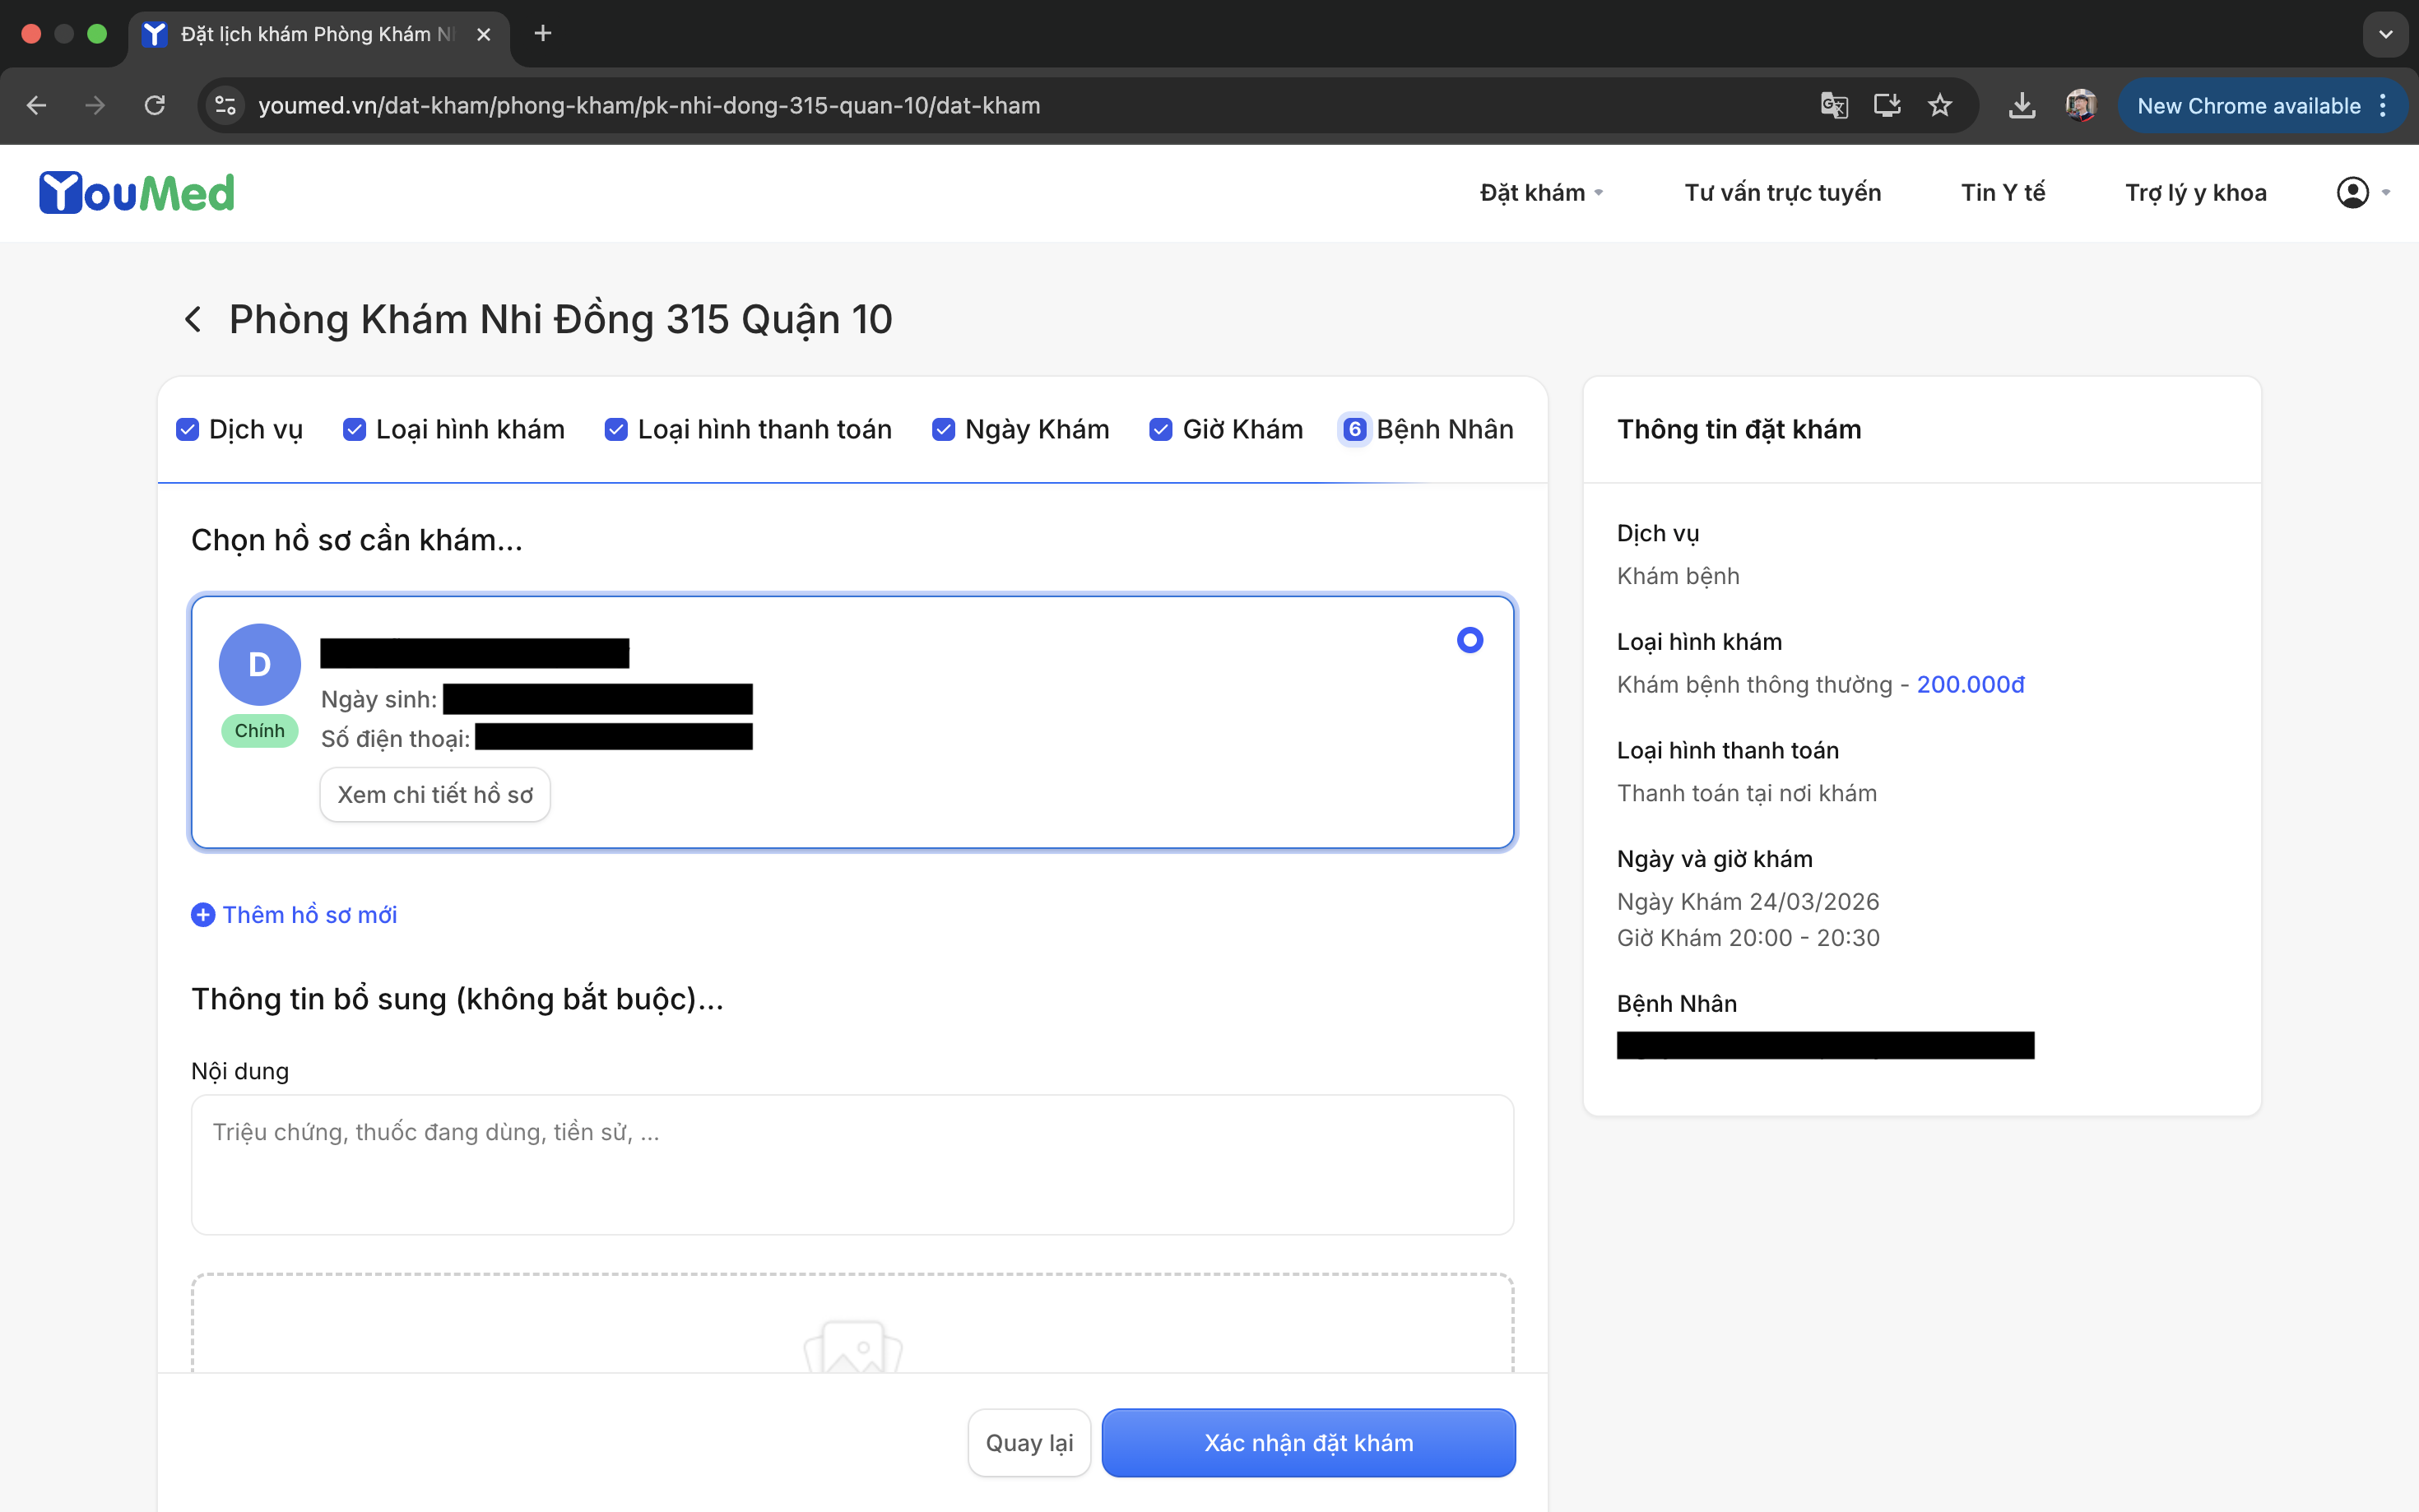
\includegraphics[width=0.85\linewidth]{images/youmed/youmed4.png}
            \caption{Clinic Appointment Scheduling}
            \label{fig:youmed_scheduling}
        \end{figure}
        
        \item \textbf{Phase 3: Billing and Confirmation} \par
        \textbf{In-App Payment Execution:} If the user chooses to pay over the app (e.g., prepaying for a private doctor's consultation online), they are routed through the platform's secure digital payment gateway to authorize and complete the transaction directly from their device. \par
        \textbf{Finalizing the  Appointment:} Once the financial transaction is authorized (for in-app payments) or officially recorded as pending (for cash on arrival), the system confirms the booking, displaying the appointment information as well as the total service fee.
        \begin{figure}[H]
            \centering
            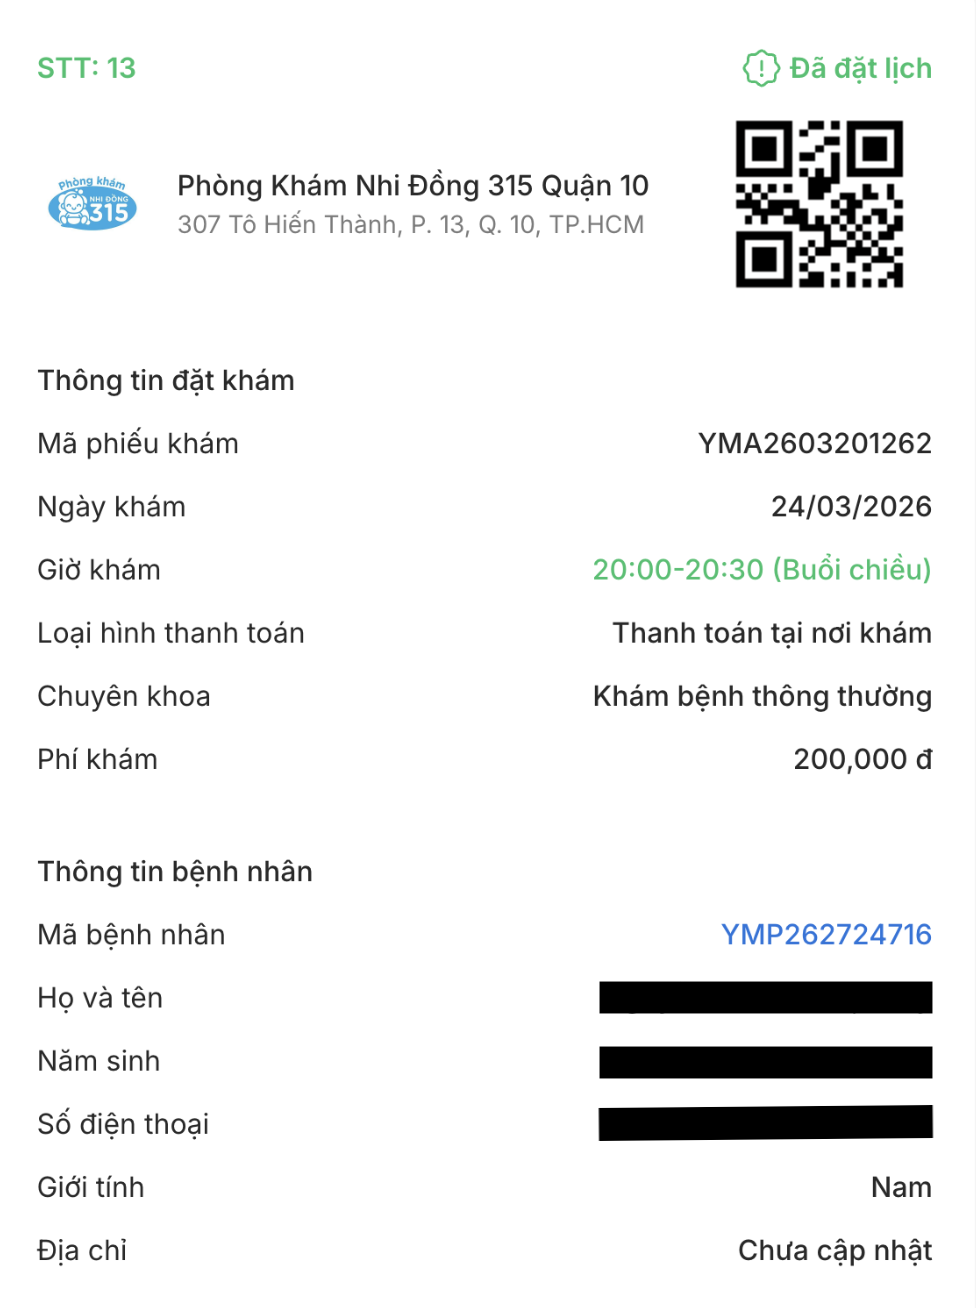
\includegraphics[width=0.4\linewidth]{images/youmed/youmed5.png}
            \caption{Appointment Confirmation}
            \label{fig:youmed_schedule_confirmation}
        \end{figure}
    \end{itemize}

    \item \textbf{Provider Workflow (Doctor Workspace)}
    \begin{itemize}
        \item \textbf{Phase 1: Account Registration and Profile Setup} \par
        \textbf{Basic Registration:} The doctor initiates the account creation by providing mandatory contact and identification details: full name, phone number, and email address. Then, the doctor specifies their practice type, choosing whether they operate independently or are affiliated with a specific clinic. The doctor uploads a professional avatar or a clinic logo for their profile. \par
        \begin{figure}[H]
            \centering
            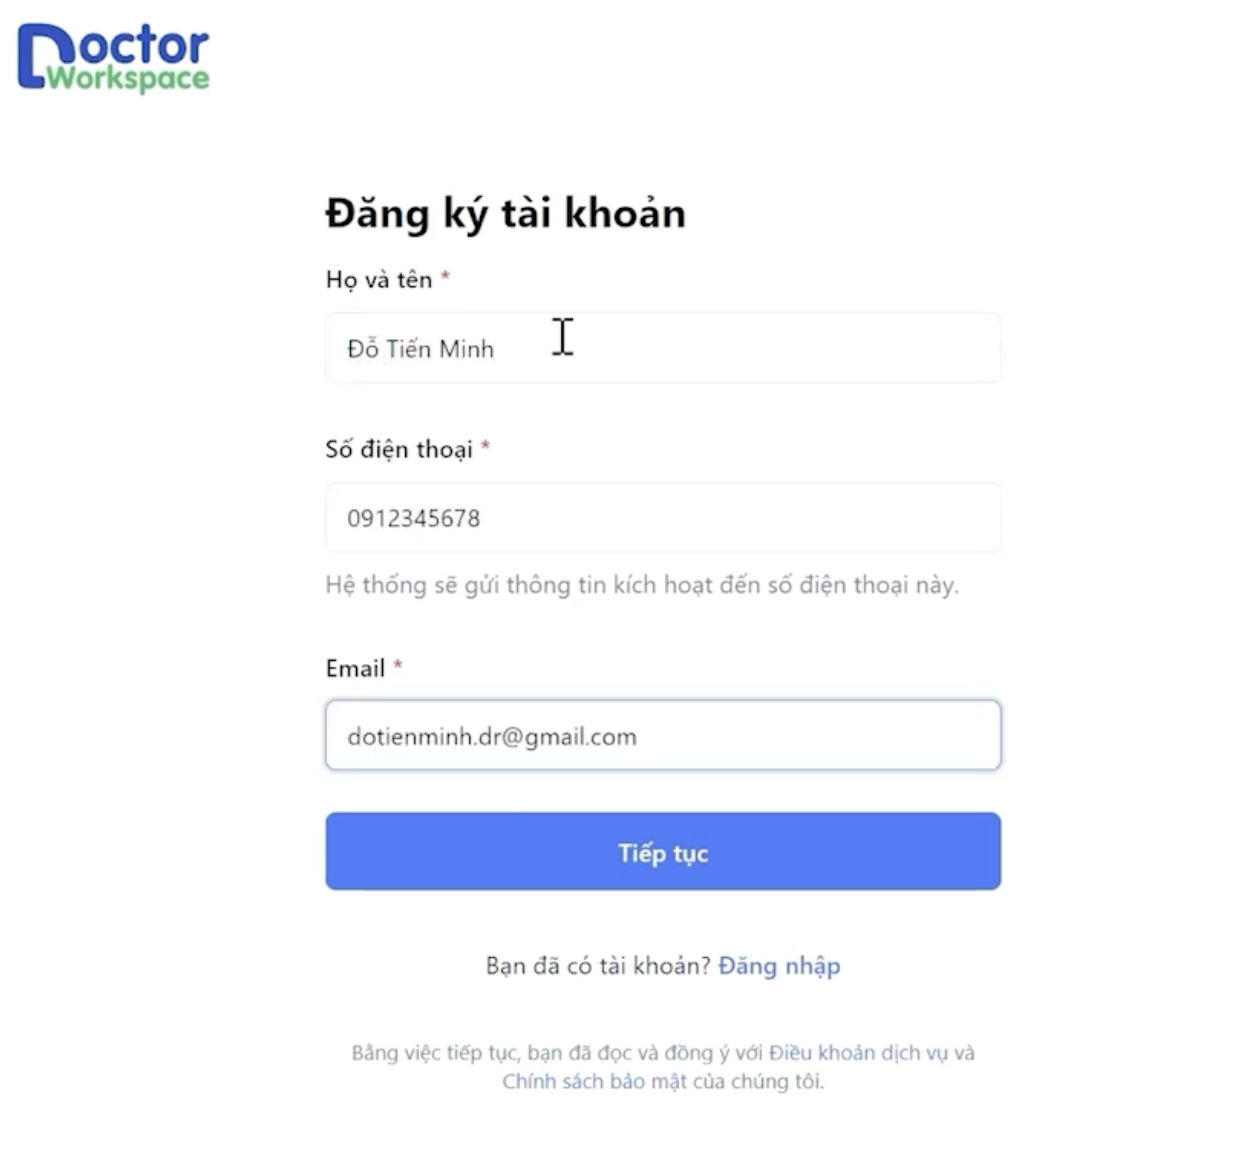
\includegraphics[width=0.4\linewidth]{images/youmed/youmed6.png}
            \caption{Doctor Workspace Account Registration}
            \label{fig:dr_registration}
        \end{figure}
        
        \textbf{Clinic Verification (If Applicable):} If operating with a clinic, the doctor must input the facility's specific regulatory and location details, including the tax code or medical examination code, the official clinic name, and the physical clinic address.
        \begin{figure}[H]
            \centering
            
\includegraphics[width=0.4\linewidth]{images/youmed/youmed7.png}
            \caption{Clinic Verification}
            \label{fig:dr_verification}
        \end{figure}

        \item \textbf{Phase 2: Update Clinic Information} \par
        The doctor improves their clinic profile by adding their full name, year of practice start, specialty, areas of expertise, workplace, position, academic title/degree, description of professional qualifications, address, service price list, training institution, introduction, work experience, awards/research projects, professional license, and image (if any).
        \begin{figure}[H]
            \centering
            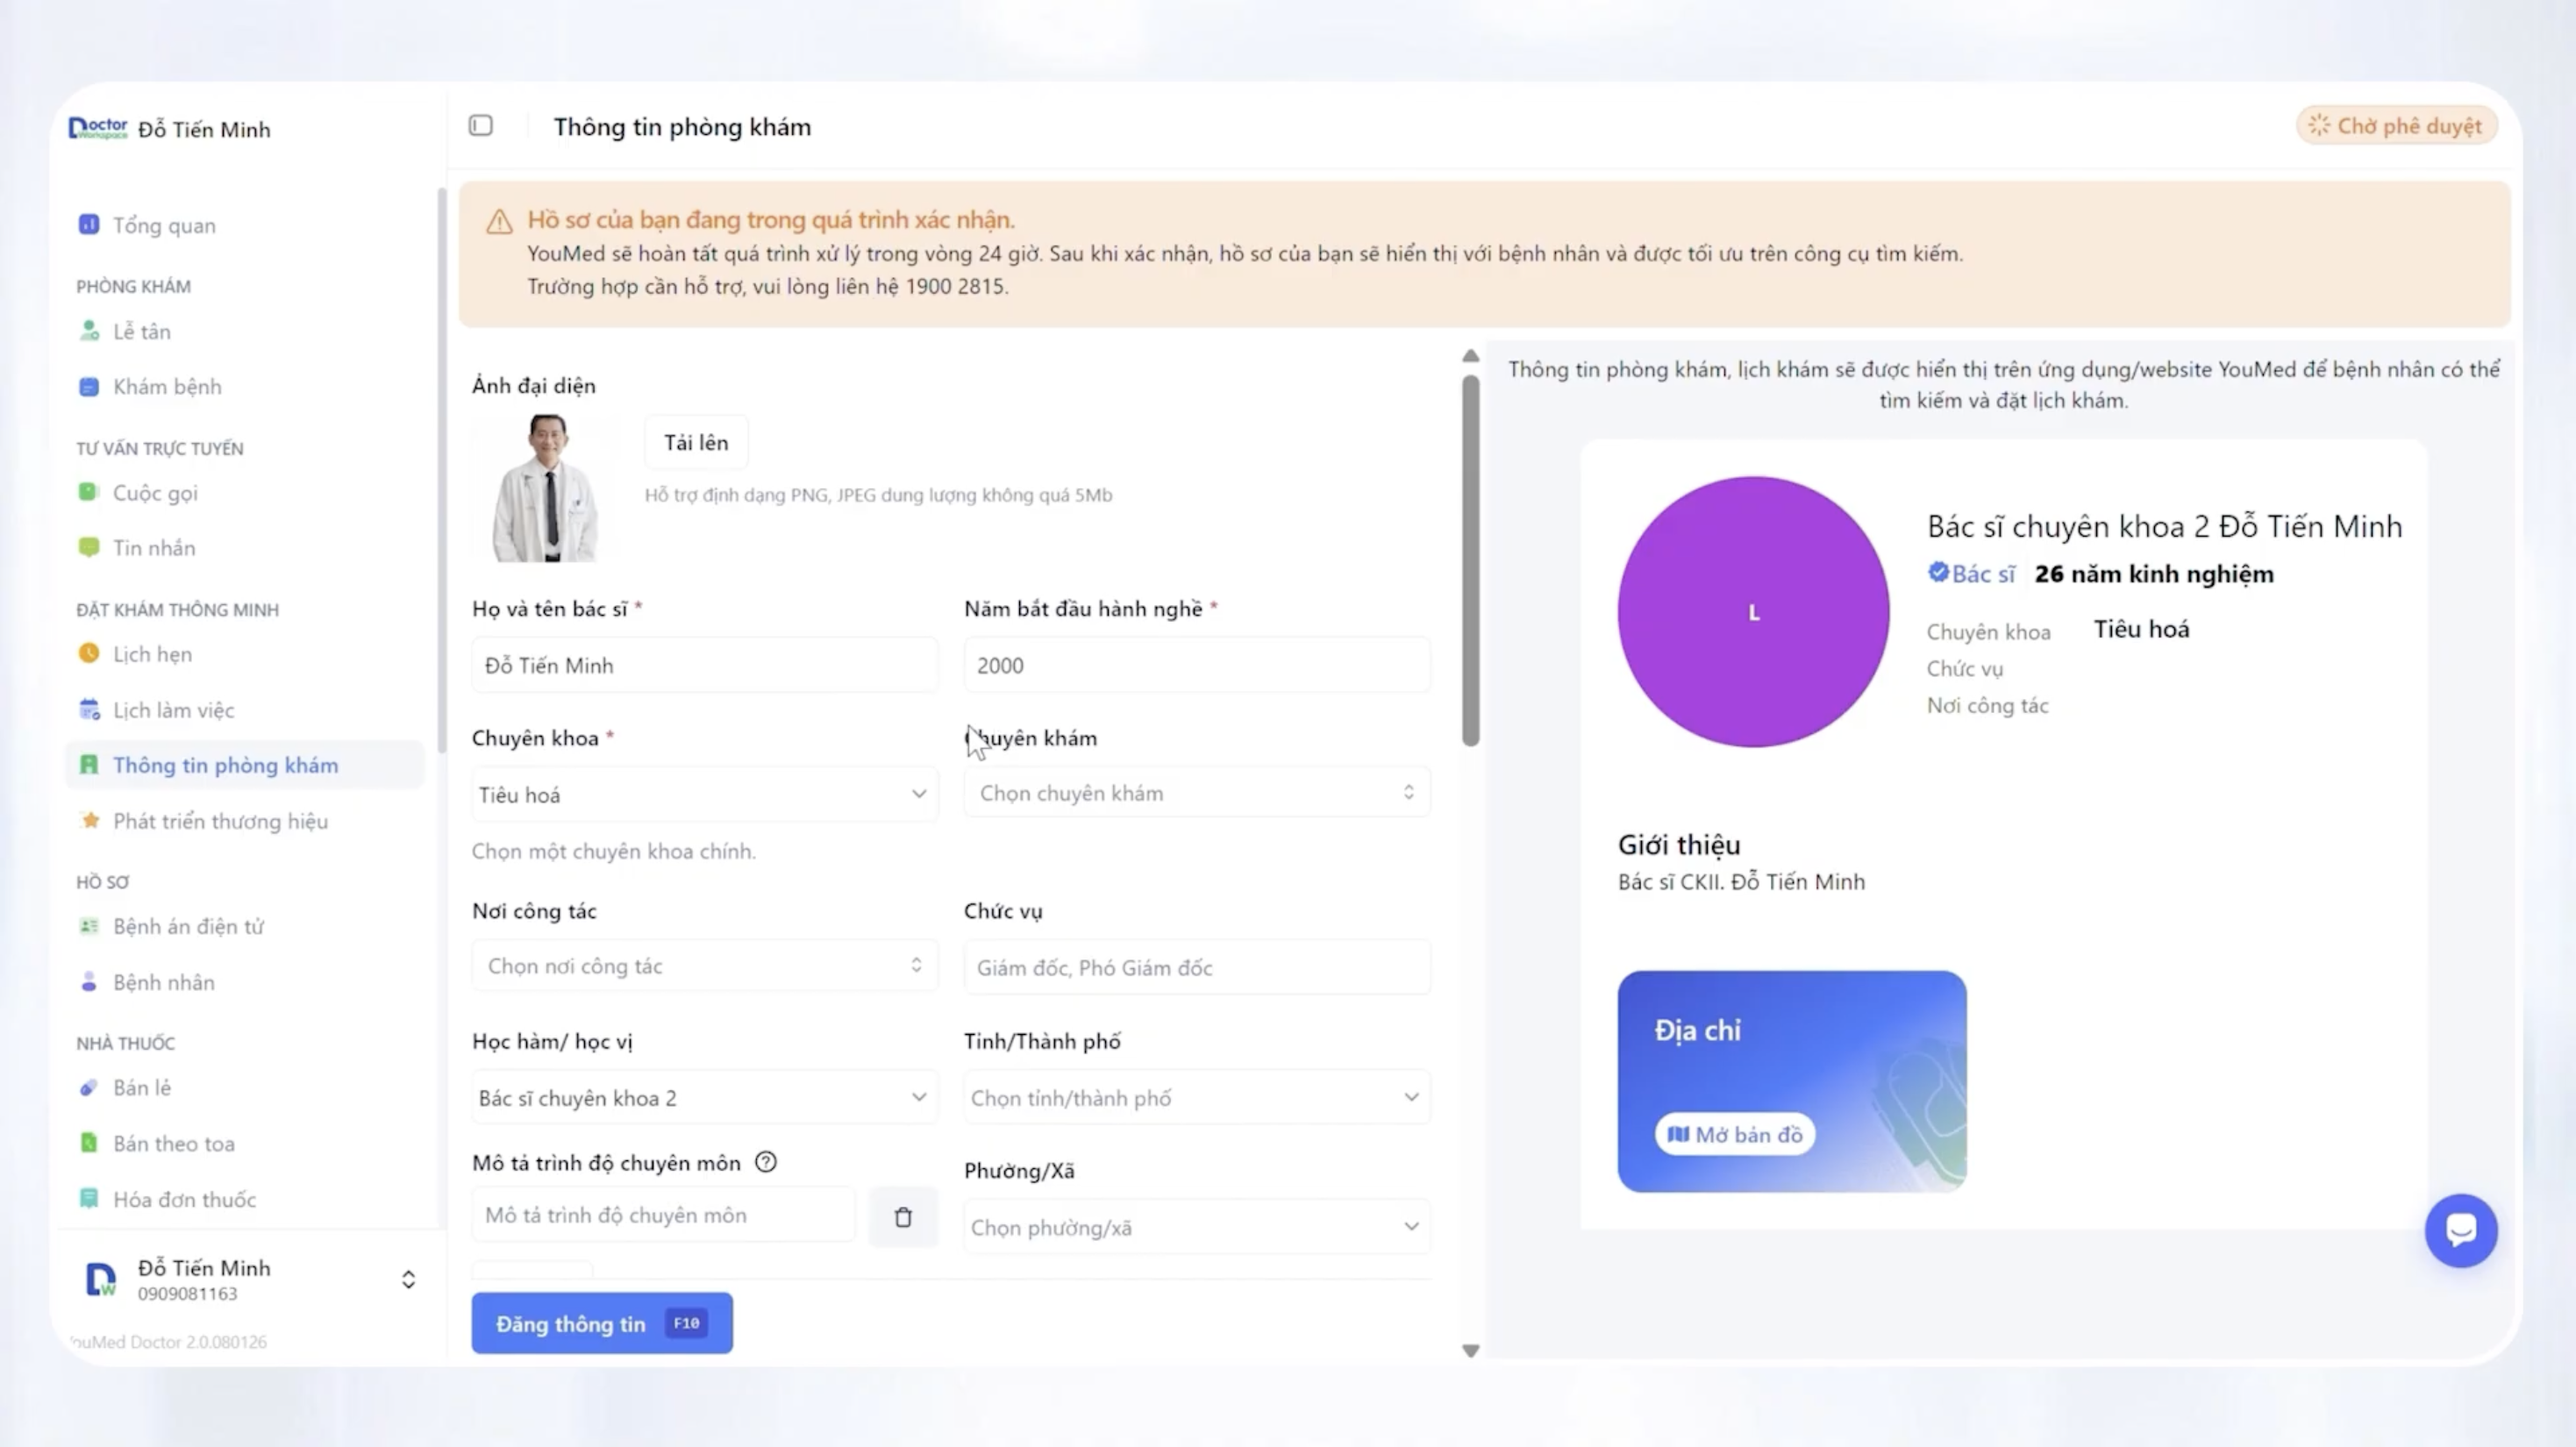
\includegraphics[width=0.9\linewidth]{images/youmed/youmed8.png}
            \caption{Update Clinic Information}
            \label{fig:dr_clinic_info}
        \end{figure}

        \item \textbf{Phase 3: Schedule Management} \par
        Using the system's built-in scheduling tool, the doctor inputs the overall start time and end time for their daily shifts, slot duration and the maximum number of consultations allowed per slot. Once confirmed, the system automatically generates the individual, bookable time slots that will be visible to patients on the platform.
        \begin{figure}[H]
            \centering
            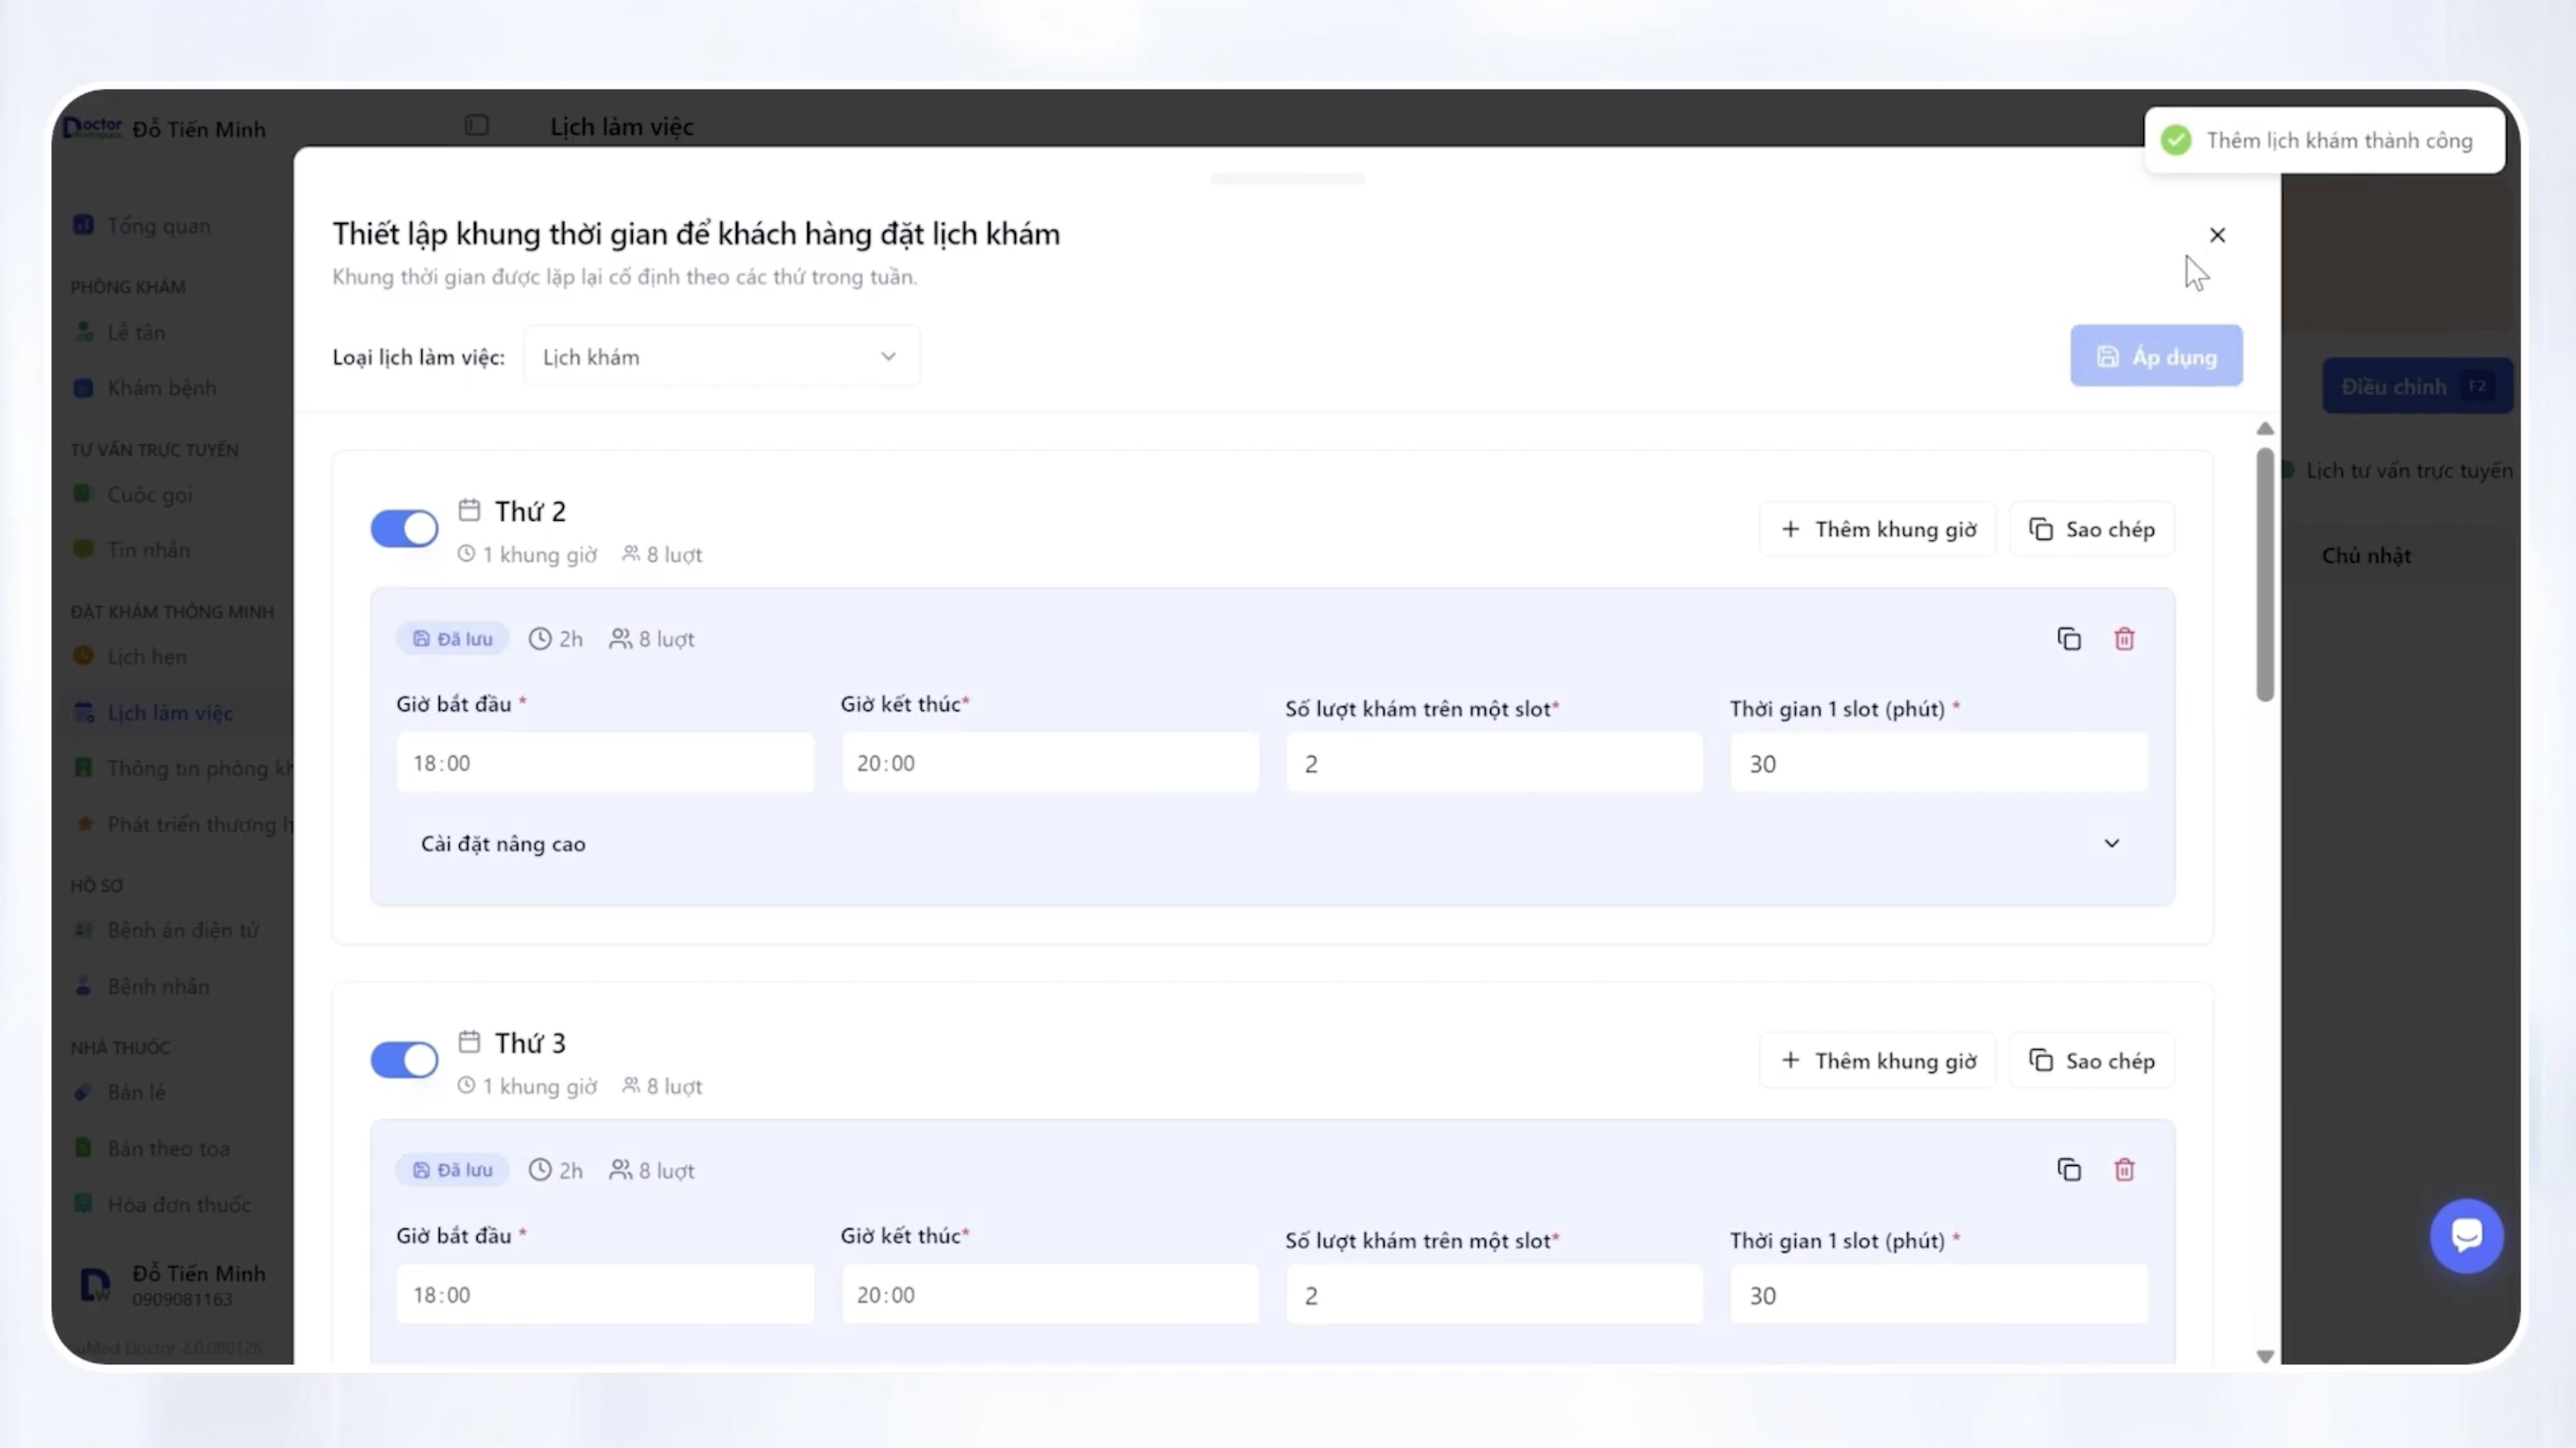
\includegraphics[width=0.9\linewidth]{images/youmed/youmed9.png}
            \caption{Schedule management}
            \label{fig:dr_schedule}
        \end{figure}

        \item \textbf{Phase 4: Patient Consultation and EMR Entry} \par
        The doctor conducts the examination, fills in the patient information, vital signs, adds any additional paraclinical orders (if any), makes a diagnosis, adds a prescription (if any), schedules a follow-up appointment (if any), and makes notes (if any).
        \begin{figure}[H]
            \centering
            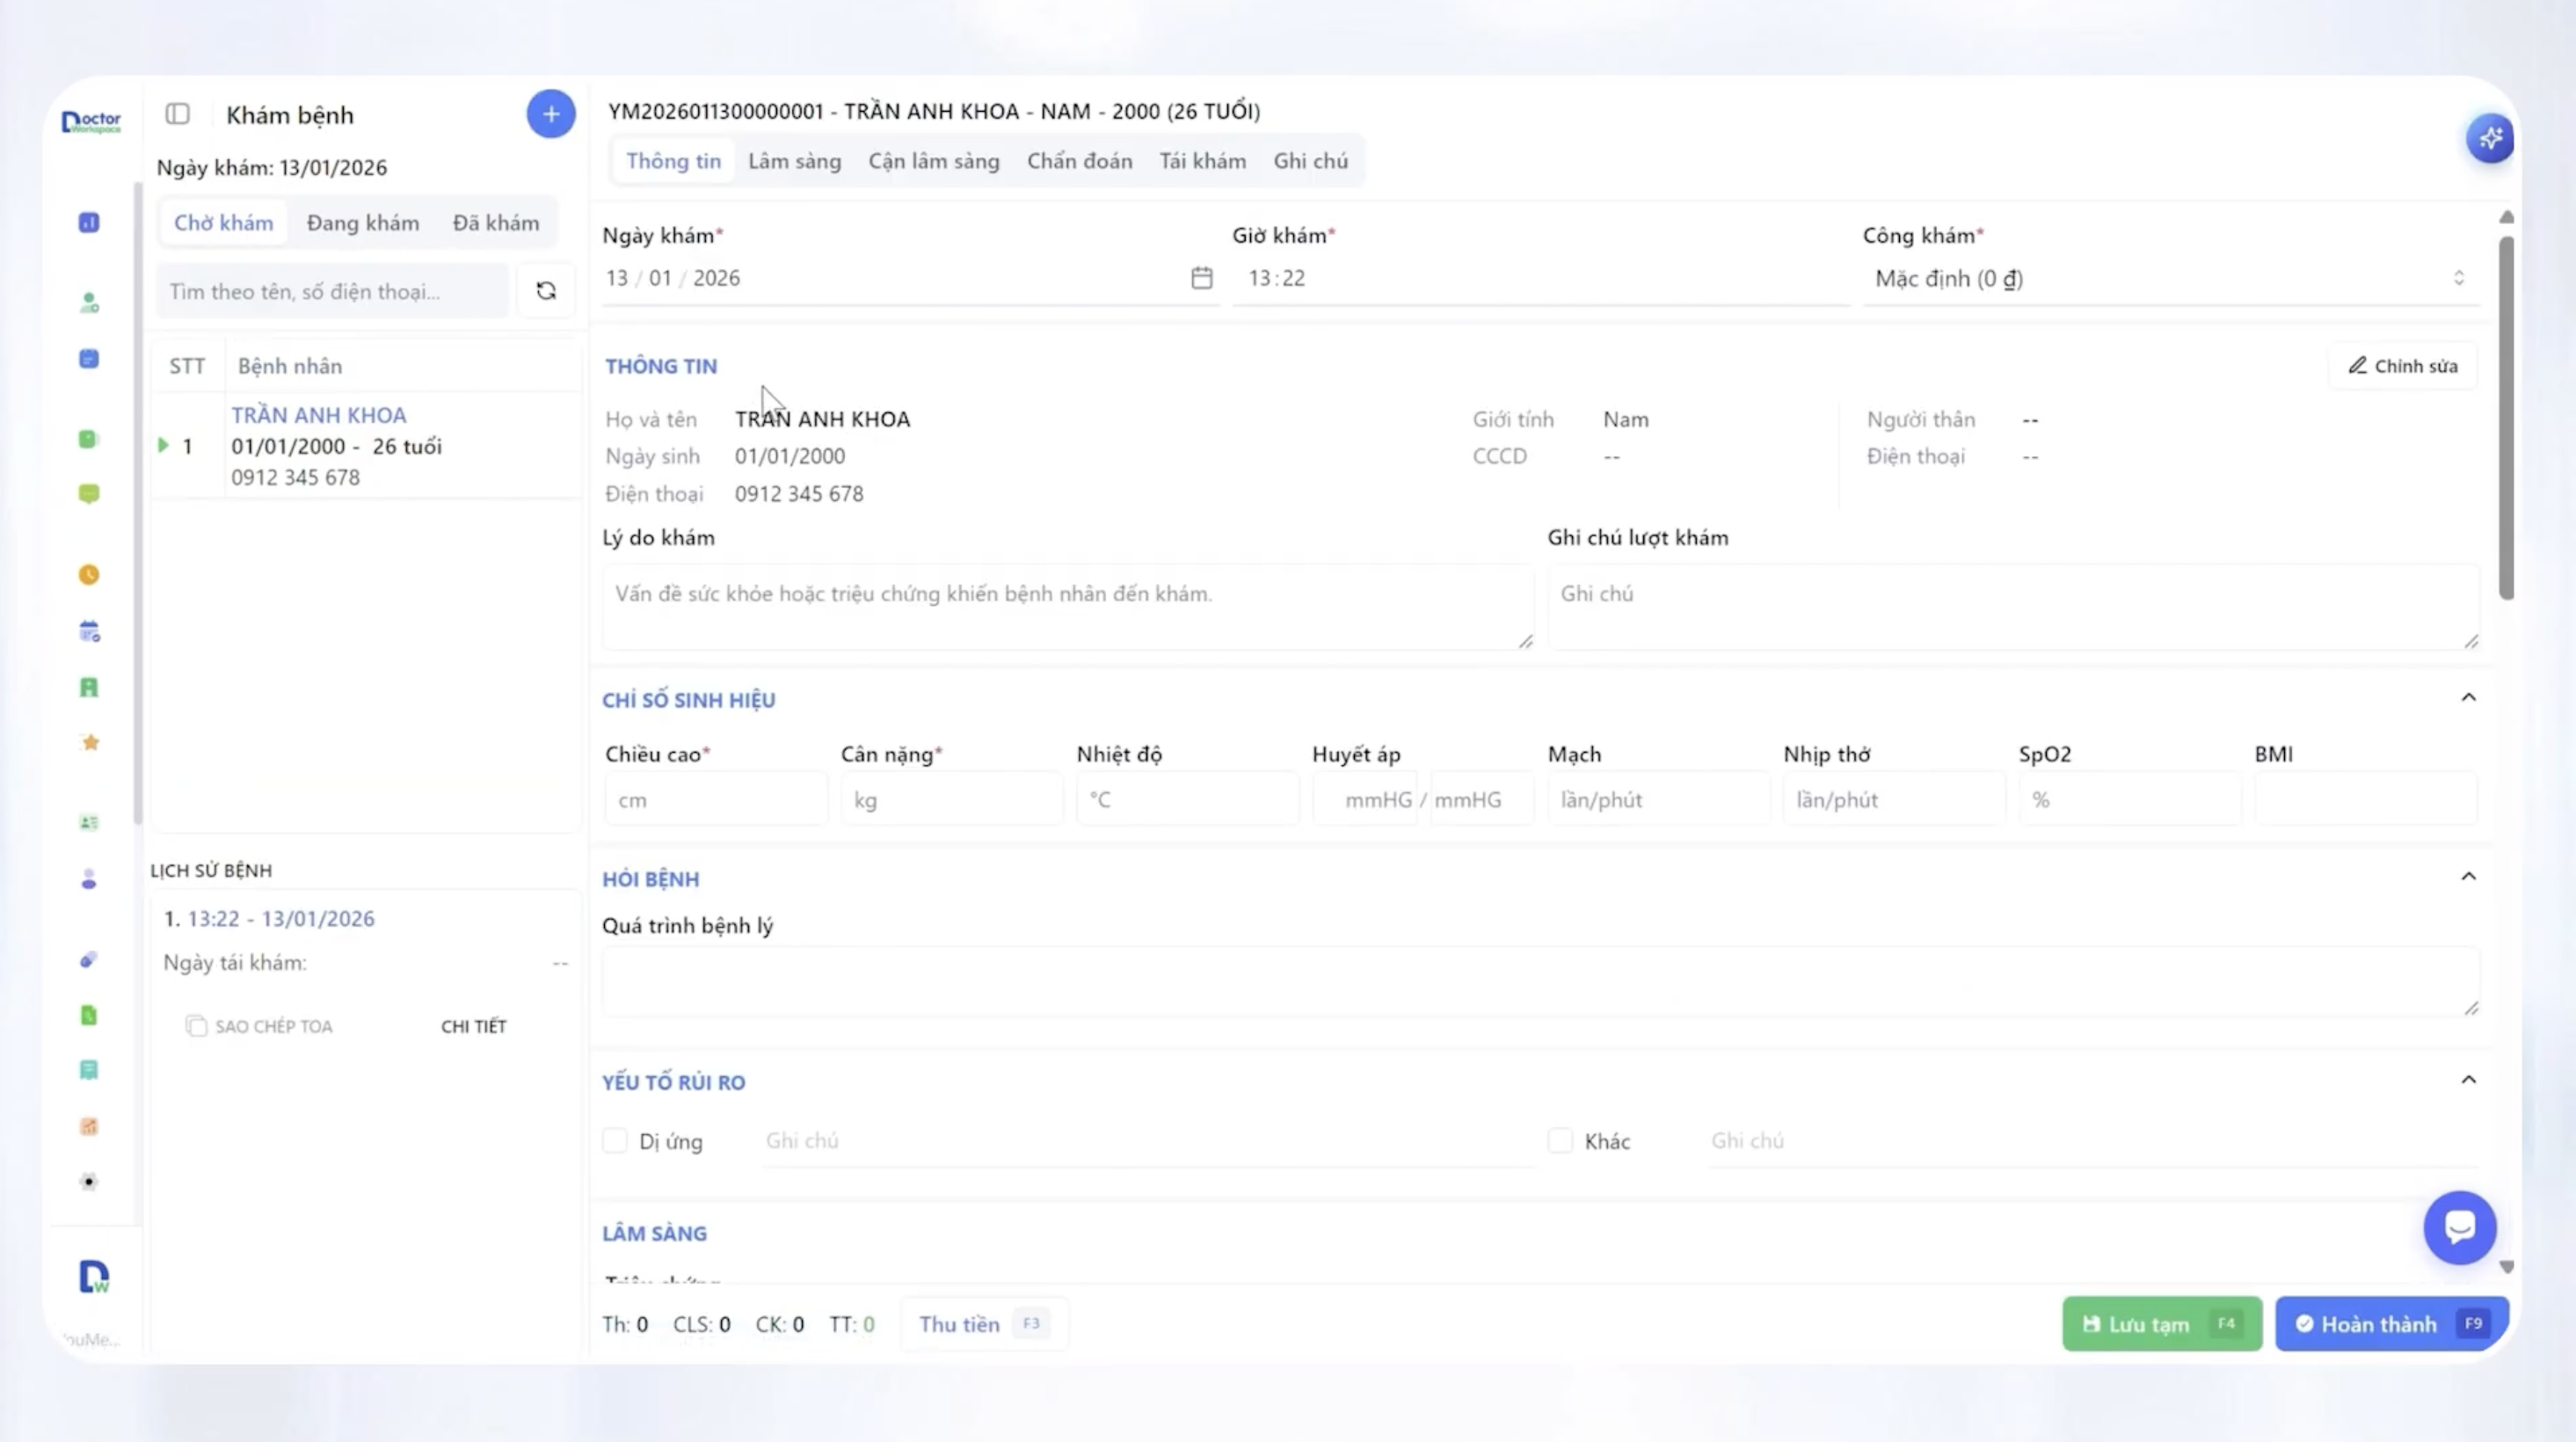
\includegraphics[width=0.9\linewidth]{images/youmed/youmed10.png}
            \caption{Patient Consultation}
            \label{fig:dr_consultation}
        \end{figure}
        
        
    \end{itemize}
\end{enumerate}

\subsection{Proposed System Description}
\textbf{System Overview:} \par
The proposed Electronic Medical Records \& Appointment System is a comprehensive platform designed to streamline healthcare access and management by connecting patients, medical professionals, and healthcare facilities. It centralizes appointment booking, doctor scheduling, and electronic medical records into a unified ecosystem. The system supports various facility types, including hospitals, clinics, and vaccination centers, operating across multiple physical branches. By allowing users to manage complex family profiles and seamlessly tracking the entire patient journey—from booking a time slot and processing billing to recording post-consultation diagnoses and prescriptions—the application ensures a cohesive, efficient, and transparent healthcare experience. \par
\textbf{User Types:}
\begin{itemize}
    \item \textbf{Customers:} End-users who register on the platform to seek medical services. They can manage multiple health profiles (for themselves and their dependents via a recursive relationship), book appointments, select preferred doctors and time slots, view billing records, and access their complete electronic medical records and prescriptions.
    \item \textbf{Doctors:} Medical professionals who provide healthcare services. They can view their assigned shifts and schedules across various facility branches, manage their daily appointments, update patient statuses, and input clinical data (diagnoses, medical records, and prescriptions) after a consultation concludes.
    \item \textbf{Administrator:} Users with elevated system privileges responsible for the operational management of the platform. They oversee user accounts, manage the registry of medical facilities and their respective branches, configure medical specialties, and handle the overall system data integrity.
\end{itemize}
\textbf{Main Functions:} 
\begin{itemize}
    \item \textbf{Account \& Family Profile Management:}
    \begin{itemize}
        \item User registration and authentication (with designated roles).
        \item Creation and management of patient profiles, including detailed demographic and insurance information.
        \item Family linking: Allowing a primary guardian account to create and manage dependent profiles (children, spouses, etc.) to book appointments on their behalf.
    \end{itemize}

    \item \textbf{Facility \& Specialty Management:}
    \begin{itemize}
        \item Displaying information for different healthcare facilities (Hospitals, Clinics, Vaccination Centers) and their multi-valued services.
        \item Managing specific physical branches, their operating hours, and hotlines.
        \item Categorizing and displaying medical specialties associated with specific doctors and branches.
    \end{itemize}

    \item \textbf{Doctor Scheduling \& Availability Tracking:}
    \begin{itemize}
        \item Configuring work shifts, start/end dates, and specific working days for doctors at various branches.
        \item Generating and managing daily schedules and time slots.
        \item Real-time tracking of time slot availability and current booked counts to prevent overbooking.
    \end{itemize}

    \item \textbf{Appointment Booking System:}
    \begin{itemize}
        \item Allowing customers to search for services/specialties and book appointments for any profile under their account.
        \item Selecting a specific time slot, assigning a doctor, and inputting pre-consultation symptom notes.
    \end{itemize}

    \item \textbf{Billing \& Payment Processing:}
    \begin{itemize}
        \item Generating billing records/invoices linked to appointments.
        \item Tracking total service fees, payment methods, and payment statuses.
    \end{itemize}

    \item \textbf{Electronic Medical Records (EMR) \& Prescriptions:}
    \begin{itemize}
        \item Creating post-consultation medical records containing diagnoses and clinical notes.
        \item Generating detailed prescriptions linked to the medical record, including specific medications, dosages, and usage instructions.
    \end{itemize}
\end{itemize}

\subsection{Detailed Data Description}
\begin{sloppypar}
    The system manages \textbf{USER\_ACCOUNT}s, which are strictly categorized as \textbf{ADMINISTRATOR}s, \textbf{DOCTOR}s, or \textbf{CUSTOMERS}. Each user account has a \textbf{\textit{\uline{unique ID}}}, a \textbf{\textit{password hash}}, a \textbf{\textit{phone number}}, an \textbf{\textit{email}}, \textbf{\textit{full name}}, and a \textbf{\textit{designated role}}.

\par A \textbf{CUSTOMER} is a specific type of account that inherits all attributes from the user account and includes an additional optional \textbf{\textit{referrer code}}. A user may create and manage multiple \textbf{PROFILE}s, representing either themselves or their family members. Each profile is uniquely identified by a \textbf{\textit{\uline{profile ID}}} and stores a \textbf{\textit{full name}}, a \textbf{\textit{phone number}}, a \textbf{\textit{date of birth}}, a \textbf{\textit{gender}}, a \textbf{\textit{complex address}} (consisting of \textbf{\textit{province/city}}, \textbf{\textit{district/county}}, \textbf{\textit{ward/commune}}, and \textbf{\textit{street detail}}), an \textbf{\textit{SSN}}, \textbf{\textit{ethnicity}}, \textbf{\textit{job}}, a \textbf{\textit{health insurance code}}, and an \textbf{\textit{email}}.

\par To manage family structures, the system implements a recursive relationship on the \textbf{PROFILE} entity, where one profile can be related to multiple other profiles. This relationship acts as a link between a primary account holder’s profile (acting as a guardian) and their dependents. Within this connection, the system captures a specific \textbf{\textit{relationship type}} (such as parent, child, or spouse) to define the nature of the bond. To ensure data consistency, the system automatically initializes a primary \textbf{PROFILE} for the user immediately upon registration, which then serves as the root for any subsequent family profiles added to the account.

\par For \textbf{DOCTOR}s, the system stores a \textbf{\textit{medical license number}}, \textbf{\textit{degree/title}}, \textbf{\textit{years of experience}}, \textbf{\textit{position}}, \textbf{\textit{biography}}, and \textbf{\textit{specialized examination}}. \textbf{ADMINISTRATOR}s hold elevated system privileges. The system tracks \textbf{MEDICAL\_SPECIALTIE}s, each having a \textbf{\textit{\uline{unique specialty ID}}}, a \textbf{\textit{name}}, and a \textbf{\textit{description}}. A doctor may possess multiple specialties, and a specialty may be associated with many doctors.

\par The system maintains a registry of \textbf{MEDICAL\_FACILITIE}s, classified as \textbf{HOSPITAL}s, \textbf{CLINIC}s, or \textbf{VACCINATION\_CENTER}s. A facility has a \textbf{\textit{\uline{unique facility ID}}}, a \textbf{\textit{brand name}}, an \textbf{\textit{introduction}}, a \textbf{\textit{website URL}}, and a multi-valued list of \textbf{\textit{services}}, each consisting of a \textbf{\textit{service name}} and its corresponding \textbf{\textit{price}}. To manage physical locations, each facility may operate multiple \textbf{BRANCH}es, each having a \textbf{\textit{\uline{unique branch ID}}}, a \textbf{\textit{specific physical address}}, a \textbf{\textit{hotline number}}, and \textbf{\textit{operating hours}}. A facility offers multiple specialties across its branches.

\par If the facility is a \textbf{HOSPITAL}, it includes a multi-valued list of \textbf{\textit{technical links}}. If it is a \textbf{CLINIC}, it does not require additional specific attributes beyond those inherited from the facility. A \textbf{VACCINATION\_CENTER} manages multi-valued \textbf{\textit{vaccine inventory records}}. Doctors work at multiple branches, and a branch may host many doctors. When associated with a branch, the system captures their \textbf{\textit{specific working days}}, \textbf{\textit{shift times}} at that particular location, \textbf{\textit{start date}} and \textbf{\textit{end date}}.

\par To manage availability, each \textbf{BRANCH} hosts multiple \textbf{SCHEDULE}s. Each schedule has a \textbf{\textit{\uline{unique schedule ID}}}, a \textbf{\textit{date}}, a \textbf{\textit{start time}}, an \textbf{\textit{end time}}, a \textbf{\textit{slot duration}}, and a \textbf{\textit{maximum number of patients per slot}}. A schedule serves as a template for multiple \textbf{TIME\_SLOT}s. A \textbf{TIME\_SLOT} is a weak entity subordinate to a schedule, uniquely identified by the combination of its \textbf{\textit{\uline{parent schedule ID}}} and a \textbf{\textit{\uline{slot number}}}. Each \textbf{TIME\_SLOT} records a \textbf{\textit{slot start time}}, a \textbf{\textit{slot end time}}, and a \textbf{\textit{status}} indicating its current availability. Additionally, each \textbf{TIME\_SLOT} maintains a \textbf{\textit{current bookings}}, which is a derived attribute calculated by totaling the number of \textbf{APPOINTMENT}s successfully linked to that specific slot.

\par The core of the platform is the \textbf{APPOINTMENT}. A profile may book multiple appointments, but each appointment has a \textbf{\textit{\uline{unique appointment ID}}} and belongs to exactly one profile. Every appointment is linked to exactly one \textbf{TIME\_SLOT}, which implicitly determines the branch and time of the visit. While the branch is determined by the slot, an appointment must also be assigned to one or more \textbf{DOCTOR}s and may require a specific \textbf{MEDICAL\_SPECIALTY}. An appointment requires a \textbf{\textit{date}} and \textbf{\textit{time}}, and may optionally include a \textbf{\textit{service type}}. \textbf{\textit{Symptom notes}} are stored as a multi-valued attribute.

\par Each appointment is linked to a distinct \textbf{BILLING\_RECORD} (or invoice), which has a \textbf{\textit{\uline{unique billing record ID}}}, a \textbf{\textit{total service fee}}, a \textbf{\textit{payment method}}, a \textbf{\textit{payment status}}, and a \textbf{\textit{transaction timestamp}}.

\par Once a consultation concludes, the system generates a \textbf{MEDICAL\_RECORD} with a \textbf{\textit{\uline{unique medical record ID}}}. A \textbf{MEDICAL\_RECORD} is linked to exactly one appointment and captures the \textbf{\textit{diagnosis}}, \textbf{\textit{clinical notes}}, \textbf{\textit{date of issuance}}, and an \textbf{\textit{edit status}}. A doctor may append a \textbf{PRESCRIPTION} (\textbf{\textit{\uline{unique prescription ID}}}) to the \textbf{MEDICAL\_RECORD}. A \textbf{PRESCRIPTION} contains multiple \textbf{PRESCRIPTION\_DETAIL}s. A \textbf{PRESCRIPTION\_DETAIL} is a weak entity identified by a \textbf{\textit{\uline{detail number}}} and its \textbf{\textit{\uline{parent prescription ID}}}, tracking the \textbf{\textit{medication}}, \textbf{\textit{dosage}}, \textbf{\textit{frequency}}, and \textbf{\textit{usage instructions}}.
\end{sloppypar}

\subsection{Semantic Constraints}
\begin{sloppypar}
    \begin{enumerate}
    \item \textbf{Capacity Hard-Limit:} 
    The derived attribute \textbf{\textit{current booked count}} of a \textbf{TIME\uline{ }SLOT} must strictly be less than or equal to the \textbf{\textit{maximum number of patients per slot}} of its parent \textbf{SCHEDULE}. The system must reject any \textbf{APPOINTMENT} insertion that would exceed this limit.

    \item \textbf{Dependent Age Validation:} 
    In the recursive relationship of the \textbf{PROFILE} entity, if a dependent profile is linked to a primary guardian profile with the \textbf{\textit{relationship type}} of "child", the system must verify the \textbf{\textit{date of birth}} attribute to ensure the dependent's age is logically valid relative to the guardian's age.

    \item \textbf{Specialty Consistency:} 
    If an \textbf{APPOINTMENT} requires a specific \textbf{MEDICAL\uline{ }SPECIALTY}, then any \textbf{DOCTOR} assigned to that appointment must possess this exact specialty.

    \item \textbf{Shift-Branch Alignment:} 
    A \textbf{DOCTOR} can only be assigned to an \textbf{APPOINTMENT} if they have a valid working schedule at the \textbf{BRANCH} implicitly determined by the appointment's \textbf{TIME\uline{ }SLOT}. Furthermore, the appointment's \textbf{\textit{date}} and \textbf{\textit{time}} must fall within the doctor's valid \textbf{\textit{start date}}, \textbf{\textit{end date}}, \textbf{\textit{working days}}, and \textbf{\textit{shift times}} at that specific branch.

    \item \textbf{Record Immutability:} 
    Based on the \textbf{\textit{edit status}} attribute of a \textbf{MEDICAL\uline{ }RECORD}, once a record is marked as concluded, the \textbf{\textit{diagnosis}} and \textbf{\textit{clinical notes}} attributes become read-only and cannot be modified to maintain legal medical integrity.

    \item \textbf{Role-Based Medical Access:} 
    A \textbf{DOCTOR} is only permitted to create or access a \textbf{MEDICAL\uline{ }RECORD} for a specific \textbf{PROFILE} if there is an existing, valid \textbf{APPOINTMENT} explicitly linking the doctor and the patient profile.

    \item \textbf{Time Slot Boundaries:} 
    For each \textbf{TIME\uline{ }SLOT}, its \textbf{\textit{slot start time}} and \textbf{\textit{slot end time}} must fall strictly within the \textbf{\textit{start time}} and \textbf{\textit{end time}} boundaries of its parent \textbf{SCHEDULE}.

    \item \textbf{Primary Profile Initialization Limit:} 
    Each \textbf{USER\uline{ }ACCOUNT} is restricted to exactly one automatically initialized primary \textbf{PROFILE} upon registration. This primary profile acts as the sole root for any subsequent family profiles added via the recursive relationship.

    \item \textbf{Appointment - Billing Record Synchronization:} 
    Each \textbf{APPOINTMENT} must be linked to exactly one distinct \textbf{BILLING\uline{ }RECORD}. The system prohibits the creation of a new \textbf{BILLING\uline{ }RECORD} if the appointment is already associated with an existing invoice.

    \item \textbf{Prescription Association Rule:} 
    A \textbf{PRESCRIPTION} (and its constituent \textbf{PRESCRIPTION\uline{ }DETAIL}s) can only be created and attached if a \textbf{MEDICAL\uline{ }RECORD} has been successfully generated following the conclusion of an \textbf{APPOINTMENT}.

    \item \textbf{Advance Booking Lead Time:} 
    An \textbf{APPOINTMENT} must be created before 4:00 PM on the day prior to its \textbf{\textit{date}}. Same-day registrations are strictly prohibited by system logic to ensure resource allocation.

    \item \textbf{Cancellation and Refund Policy:} 
    An \textbf{APPOINTMENT} can only be cancelled, and a \textbf{BILLING\uline{ }RECORD} refund triggered, if the cancellation occurs before 4:30 PM on the day preceding the appointment \textbf{\textit{date}}. Cancellations after this threshold do not trigger automated refunds.
\end{enumerate}    
\end{sloppypar}